
%% PRAEAMBEL
\documentclass[a4paper,12pt]{article}
%\usepackage{amsmath,amssymb,amsthm}
\usepackage{mathtools}
\usepackage{graphicx}
\usepackage{ucs}
\usepackage[utf8]{inputenc}
\usepackage{microtype}
\usepackage[ngerman,english]{babel} 
\usepackage{rotating}
\usepackage{float}
\usepackage{placeins}
\usepackage{cite}
\usepackage{color}
\usepackage{listings}
\usepackage[table,xcdraw]{xcolor}
\parindent 0pt % keine Einrückung am Anfang jedes Absatzes
\definecolor{dkgreen}{rgb}{0,0.6,0}
\definecolor{gray}{rgb}{0.5,0.5,0.5}
\definecolor{bluekeywords}{rgb}{0.13,0.13,1}
\definecolor{lightbluecomments}{rgb}{0.545,0.490,0.420}
\definecolor{redstrings}{rgb}{0,0.5,0}
\usepackage[left=25mm,top=29mm,bottom=29mm,right=25mm,headheight=15mm,headsep=10mm,footskip=10mm]{geometry}
\usepackage{setspace}
\usepackage{lastpage}
\usepackage{subcaption}
\usepackage{caption}

% Programmeinbindung 
\usepackage{listings} % für C Programm Einbindung
\lstloadlanguages{Matlab}
\lstset{language=Matlab, showspaces=false,
				   showtabs=false,
				   breaklines=true,
				   showstringspaces=false,
				   breakatwhitespace=true,
				   escapeinside={(*@}{@*)},
				   commentstyle=\color{lightbluecomments},
				   keywordstyle=\color{bluekeywords},
				   stringstyle=\color{redstrings},
				   basicstyle=\ttfamily,
				   numbers=left,
				   stepnumber=1,
				   numberstyle=\small
      }




\onehalfspacing
%////////////////////////////////////////
%Kopfzeile:
\usepackage{fancyhdr}
\addtolength{\headheight}{1.5cm} % make more space for the header
\pagestyle{fancyplain} % use fancy for all pages except chapter start
%\lhead{\includegraphics[height=1.3cm]{logo2}} % left logo
\rhead{
\includegraphics[height=1.0cm]{TUlogo.png}} % right logo

\fancyhead[L]{\today}
\fancyhead[C]{PROTOCOL}
\renewcommand{\headrulewidth}{1pt} % remove rule below header
%foot
\fancyfoot[R] {\thepage \space von \pageref{LastPage}} % SEITENANZAHL AENDERN
\fancyfoot[C]{}
%\fancyfoot[L]{Datei: Protokoll\_ Gruppe\_ 2\_ Filter.tex}

%///////////////////////////////
%\title{VU Modeling and Simulation}
\date{\vspace{-10ex}}
% --------------------------------------------------------- BEGIN DOCUMENT ------------------------------------------------------------------------

\begin{document}
%\maketitle
\vspace*{10mm}
\begin{center}
\huge{\textbf{VU Modeling and Simulation}} \\
\vspace{20mm}
\Large{\textbf{Cellular Automaton vs. Difference Equation}}\\
\textbf{Case Study: Predator Prey System}\\ \ \\
\begin{large}
\textbf{Autoren}\\
    	Christoph Hämmerle\\
    	Philipp Ganiu\\
    	Jennifer Lumetzberger\\
\end{large}   	
\end{center}

\newpage
\tableofcontents
\newpage
%\begin{figure}[H]
%\centering
%\includegraphics[width=0.75\textwidth]{laufRPosition}  
%\caption[kurve]{Die Abbildung zeigt die vertikale Position des rechten Fußes in Abhängigkeit von der horizontalen x-Koordinate während eines Gangzyklus (vgl. Abbildung \ref{koordinatensystem}). Die Events TO und HS sind markiert. Der Plot wurde mit den erhaltenen Daten von Lauf2.m erstellt.}
%\label{laufRPosition}
%\end{figure} 

\section{Introduction}
A forester wants to get information about the maximum number and the dynamics of the population of
deer in its forest. In order to observe the correlation between the number of red-foxes and deer, a predator-prey approach is modelled.
Different modelling concepts are compared: a cellular automata model and a formulation given by a damped version of the classic ODE model by Lotka and Volterra.\\ \ \\

\textbf{Damped Differential Equation Model} \\
First of all a difference equation model is derived (The derivation is very similar to the derivation of the
classic differential-equation model). The following is observed (e.g. by external datasets or by opinion of the forester):

\begin{itemize}
\item{During each month in the absence of a natural predator the population of deer increases by a
certain rate $\alpha >$ 0 which includes natural birth and death rates. As the forest has a certain
resource capacity M the growth is limited leading to $\alpha(M-x)$ (respectively $\alpha(M-x-y)$ if there
is a fox-species too)}
\item{During each month in the absence of any deer the population of foxes decreases by a certain rate
 $\gamma >$ 0 as the population is starving.}
\item{In case of cohabitation of the two species we could observe that the number of deer each month is
reduced by xy$\beta$ with a positive $\beta$ animals.}
\item{Benefting from fresh meat, the decreasing rate $\gamma$
 is balanced by a positive rate $\delta$x. In case $\delta x-\gamma
 > 0$
there is an increase of the number of foxes. Otherwise the number decreases.}\\
\end{itemize}
Putting all those observations together leads to the following dynamics:

\begin{center}
\begin{equation}
x_0(t) = x(t)\alpha \times(M - x(t) - y(t)) - x(t)y(t)\beta 
\label{eq:1}
\end{equation}
\begin{equation}
y'_0(t) = y(t)(\delta x(t) \gamma)
\label{eq:2}
\end{equation}
\end{center}

\textbf{Cellular Automata Model}\\
Given the same information a cellular-automata is derived.\\
\begin{itemize}
\item{We assume our forest to be approximately rectangular and apply a rectangular grid.}
\item{At the beginning of the simulation each cell of the grid is either placed a prey, a predator or left
empty. We furthermore sloppily say that a cell is either "prey", "predator" or "empty".}
\item{The whole matrix is updated simultaneously each month by the following rules:}
\begin{itemize}
\item{In case cell i,j is empty, we chose one neighboured cell at random and check if the cell is prey. In
this case, the neighboured cell reproduces and cell i,j becomes prey as well with probability $p_1$.}
\item{In case cell i,j is prey, we chose one neighboured cell at random and check if the cell is predator.
In this case, the neighboured cell eats up the prey and reproduces. Therefore cell i,j becomes
predator as well with probability $p_2$.}
\item{In case cell i,j is predator, the predator unfortunately dies with a certain probability. Therefore
cell i,j becomes empty with probability $p_3$.}
\end{itemize}
\end{itemize}

By a neighboured cell we understand any cell which is not father away as k cells from the original cell,
whereas k is a natural number.



\section{Task description}

\textbf {Task 1}\\ 
Implement the damped differential equation model and perform some trial runs. Try several self chosen
parameters $0 < \alpha,\beta,\gamma,\delta$ for the simulation and fix $x_0 = 4000$ and $y_0 = 1000$ as initial populations.
Notice that $M  \gg x_0 + y_0$ and fix a self chosen natural number for it. \\ \ \\
\textbf {Task 2}\\ 
Implement the cellular automaton (CA) model and perform some trial runs. Try some self chosen
parameters $0 < p_1, p_2, p_3 < 1$ and fix neighbourhood parameter k = 1 at the first place. Use the same
initial conditions for the CA as for the difference model and initially mark 4000 cells as prey and 1000
cells as predator - note that you need to use a rectangle with more than 4000 + 1000 cells (furthermore
denoted as N) in order to perform simulations.\\ \ \\
\textbf {Task 3}\\ 
Try to find out how to present the results of the CA in animated form and how you can aggregate the
results of the CA in order to achieve comparable curves to the differential equation.\\ \ \\
\textbf {Task 4}\\ 
Fix all other parameters and experiment with different rectangles with same number of cells. Experiment
whether the shape of the rectangle influences the results.\\ \ \\
\textbf {Task 5}\\ 
Try to find parameter-settings $(\alpha,\beta,\gamma,\delta, M)$ and $(p_1, p_2, p_3,N, k)$ so that the corresponding resulting
curves of both models look alike.\\ \ \\
\textbf {Task 6}\\ 
Summarize your project work as a protocol.\\ 


\section{Methods}
The predator-prey approach is modelled with Matlab.

\section{Execution}
% Vorgehensweise beim Programmieren, Umsetzung, Codeschnipsel

\subsection {Task 1}
For the first task, the damped differential equation model is implemented in Matlab. \\
As initial values for the deer (x) and fox (y) population,  we take $x_0 = 4000$ and $y_0 = 1000$, as given in the task.
For the resource capacity of the wood M, we consider $M  \gg x_0 + y_0$ and fix it with $M=10000$.

The parameters $\alpha$, $\beta$, $\gamma$ and $\delta$ are also fixed with:\\ \ \\
\begin{center}
\begin{displaymath}
\begin{split}
\alpha = 0.001\\% deer growth
\beta = 0.003\\% deer reduction
\gamma = 2\\% fox decreasing 
\delta =0.001% fresh meat increase
\end{split}
\end{displaymath}
\end{center}

First of all, a matrix is created, which stores the month and the corresponding amount of deer and foxes, for every month from 0 (starting point) to the desired maximum time point:\\

\begin{table}[]
\centering
\begin{tabular}{
>{\columncolor[HTML]{EFEFEF}}l lllll}
month & \textbf{0} & 1 & 2 & ... & m \\
deer & \textbf{4000} & ? & ? & ? & ? \\
foxes & \textbf{1000} & ? & ? & ? & ?
\end{tabular}
\caption{Matrix scheme with information on amount of deer/foxes for each month}
\label{my-label}
\end{table}

Via the given difference equations (\ref{eq:1}) and (\ref{eq:2}) the population of each time point can be calculated.
After each iteration, the data is stored into the matrix.

\subsection {Task 2}

For implementing the cellular automata (CA) model, some self chosen
parameters $0 < p_1, p_2, p_3 < 1$ are used. The neighbourhood parameter k is fixed with $k= 1$ at the first place. 
As with the difference model, the inital values are the same: $x_0=4000$ and $y_0=1000$.

So, the initial parameter setting is as following:

\begin{center}
\begin{displaymath}
\begin{split}
rows = 70\\
col = 200\\
p1= 0.01\\ % probability for prey reproduction
p2= 0.8\\ % probability for predator reproduction
p3= 0.01\\ % probability for predator dying
\end{split}
\end{displaymath}
\end{center}

Now the first step is to set up a matrix with the 4000 deers and 1000 foxes randomly distributed in our rectangle (forest). The rectangle is built up by the number of rows and columns. Therefore in this case we have 14000 (70x200, universally valid: N) cells, that's why we create a row-vector \textit{initvalues} with N entries. With the function \textbf{randperm} we pick 5000 ($x_0+y_0$) cells with a random permutation between 0 and N, so each value appears only once. These random numbers we use as indices of \textit{initvalues} and assign the first 4000 ($x_0$) cells to 1 (which stands for deer). The next 1000 ($y_0$) random numbers we assign to 2 (which means foxes). Since we initialized \textit{initvalues} with zeros, the step of creating the initial population is done.\\
In order to create the rectangle, we take our \textit{initvalues} vector and fill a new matrix \textit{population} with its values, by using the \textbf{reshape} function.\\

For creating the states for each timestep, a for-loop is used, regarding each cell and applying the rules of the CA described at the beginning.

After each iteration we sum up all our foxes, deer and empty spaces, to have results which can be compared later with the values of the differential equation model.



\subsection {Task 3}
For achieving comparable results with the CA as with the differential equation, after each loop iteration, all cells belonging to the fox/deer/no population are summed up and stored in a matrix.\\

For animating the CA, a plot is created with the x-axis representing the length of our rectangle and the y-axis illustrating the width of the rectangle. Using the Matlab function \textbf{spy}, each cell of the rectangle/matrix can be marked in a different color. When updating the plot after each loop iteration (each time step), we have created a simple animation presenting the population development of our species.

\subsection {Task 4}
In Task 4 all parameters are fixed, except of the shape of the rectangle (number of cells stays the same). The results are shown in the results section.
\subsection {Task 5}
In Task 5 the parameters $\alpha,\beta,\gamma,\delta,M$ as well as $p_1, p_2, p_3,N, k$ shall be changed so that the corresponding resulting
curves of both models look alike. The results are shown in the results section.
\subsection {Task 6}
This task is obviously done.

\section{Results}
\subsection {Task 1}
When establishing the difference equation model with the parameters fixed in the execution section of Task1, we gain the following result:\\

\begin{figure}[H]
\centering
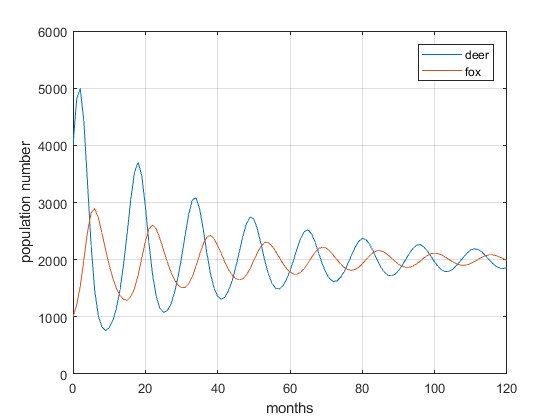
\includegraphics[width=0.75\textwidth]{Task1}  
\caption[task1]{Population development of foxes and deer over 10 years}
\label{task1}
\end{figure} 

At the beginning, the deer population is 4 times the fox population. Due to the high amount of food for the foxes, the fox population rises, which leads to a fall in the deer population. After several years, an equilibrium is found, when each species comprises about 2000 individuals. In table \ref{DE} the population numbers of certain time points can be seen.

\begin{table}[h!]
\centering
\begin{tabular}{
>{\columncolor[HTML]{EFEFEF}}l llllllll}
month & \textbf{0} & 1 & 5 & 24 & 60 & 80 & 100 & 120 \\
deer & \textbf{4000} & 4800 & 2258 & 1154 & 1806 & 2370 & 1959 & 1864 \\
foxes & \textbf{1000} & 1200 & 2817 & 1375 & 1783 & 1927 & 2116 & 1984
\end{tabular}
\caption{Difference Equation Model: Population development at certain time points }
\label{DE}
\end{table}

\subsection {Task 2 and 3}
In Task 2 and 3, the cellular automata model was created. We can compare the rectangle in the initial state with the results after 10 years. We also look at two other time steps, namely at $m_1 = 5$ months and $m_2 = 24$ months.

\begin{figure}
        \centering
        \begin{minipage}[t]{0.48\textwidth}
                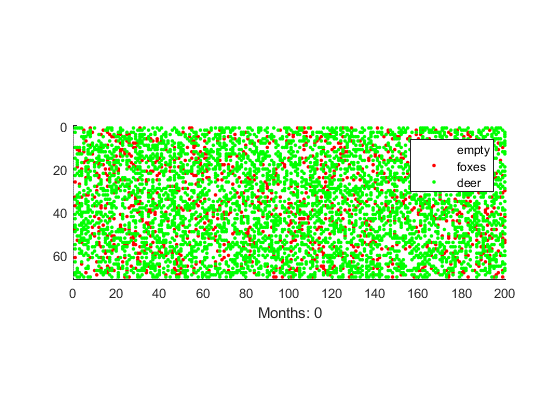
\includegraphics[width=\textwidth]{Task2starttime}
                \vspace{-20mm}
                \caption{CA at initialization time}
                \label{Task2start}
        \end{minipage}\hfill
        \begin{minipage}[t]{0.48\textwidth}
                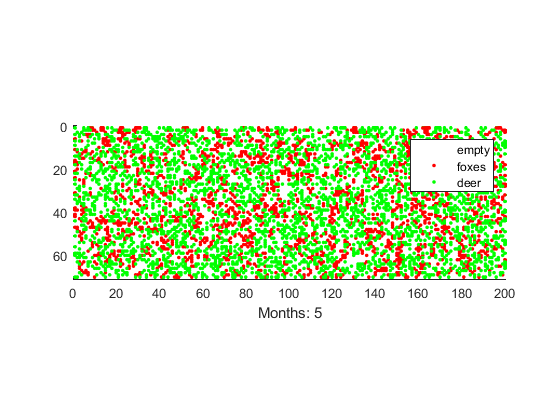
\includegraphics[width=\textwidth]{Task2month5}
                \vspace{-20mm}
                \caption{CA after 5 months}
                \label{Task2M5}
        \end{minipage}
        \medskip

        \begin{minipage}[t]{0.48\textwidth}
                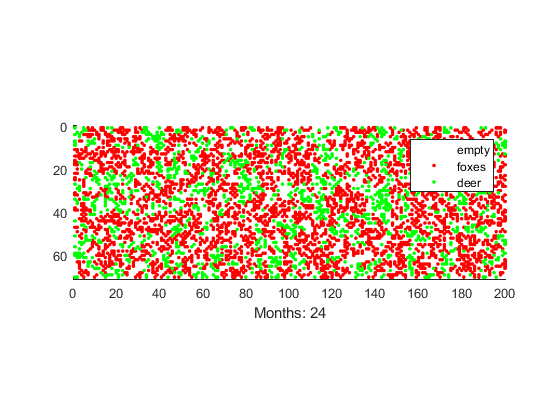
\includegraphics[width=\textwidth]{Task2month24}
                \vspace{-20mm}
                \caption{CA after 2 years}
                \label{Task2M24}
        \end{minipage}\hfill
        \begin{minipage}[t]{0.48\textwidth}
                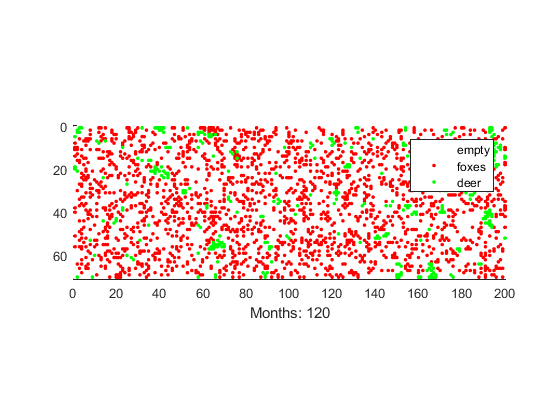
\includegraphics[width=\textwidth]{Task2endtime}
                \vspace{-20mm}
                \caption{CA after 10 years}
                \label{Task2end}
        \end{minipage}
        \medskip
\end{figure}

\newpage
As can be seen in Figure \ref{Task2start} - \ref{Task2end}, the population of deer decreases drastically with time, whereas the population of foxes increases until a certain time and then decreases again. In table\ref{CA} some values of the population development can be seen.

\begin{table}[h!]
\centering
\begin{tabular}{
>{\columncolor[HTML]{EFEFEF}}l llllllll}
month & \textbf{0} & 1 & 4 & 24 & 60 & 80 & 100 & 120 \\
deer & \textbf{4000} & 3821 & 3082 & 1190 & 540 & 440 & 405 & 403 \\
foxes & \textbf{1000} & 1191 & 1952 & 3529 & 3146 & 2707 & 2275 & 1882
\end{tabular}
\caption{Cellular Automata results at certain time points}
\label{CA}
\end{table}

The whole course of events can be seen in Figure \ref{CAgraph}.

\begin{figure}[H]
\centering
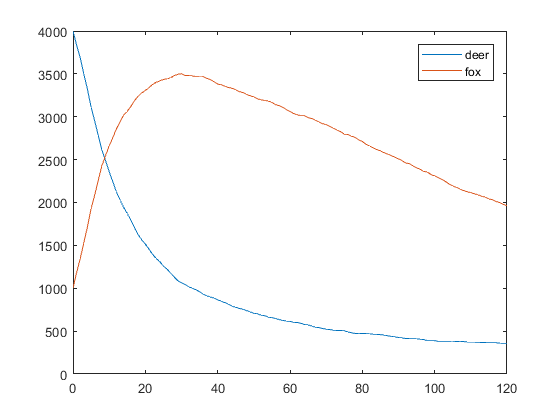
\includegraphics[width=0.75\textwidth]{CA100R140C}  
\caption[CAgraph]{Population behaviour over 10 years with CA model}
\label{CAgraph}
\end{figure} 


\subsection {Task 4}
The number of cells is fixed with N = 14000. We are only changing the shape of the rectangle and observe the results.
When we do not change the shape of the rectangle dramatically, the behaviour of the model also does not change a lot. Due to the randomly created matrix and the probability influences, each run of the code is different and cannot be repeated.
When we change the shape of the rectangle in a way in which we set one parameter (row,column) very small (to 1 or 2), the results change a lot (see Figures \ref{CAgraph2rows} and \ref{CAgraph1row}).

\begin{figure}[h!]
\centering
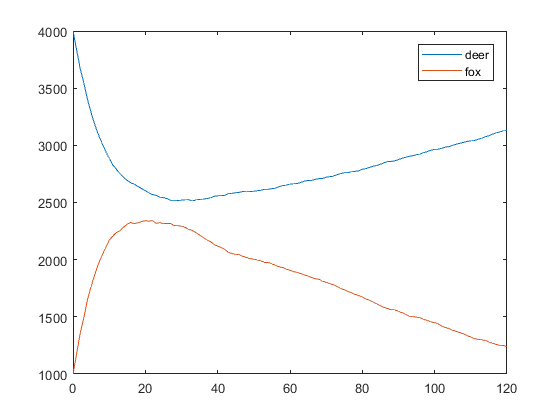
\includegraphics[width=0.75\textwidth]{CA2R7000C}  
\caption[CAgraph]{CA model with only 2 rows}
\label{CAgraph2rows}
\end{figure} 

\begin{figure}[h!]
\centering
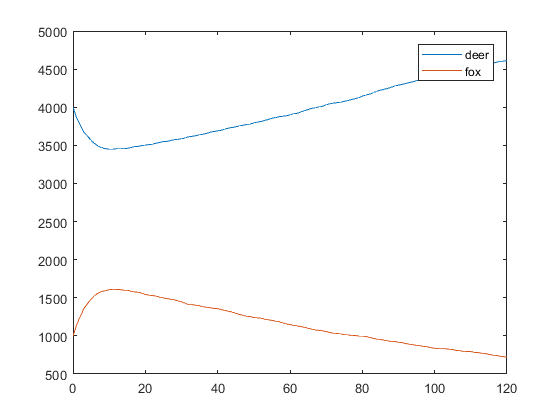
\includegraphics[width=0.75\textwidth]{CA1R14000C}  
\caption[CAgraph]{CA model with only 1 row}
\label{CAgraph1row}
\end{figure} 

\textcolor{red}{
Since the algorithm of the implemented cellular automata does not consider all neighbours, but only 1 randomly chosen neighbour, there should not be a large difference by changing the shape of the rectangle. If for example, we have a very narrow and long trail of wood (only 2 neighbours possible, or 1 at each end of the trail, when we use $k=1$), the probability for a deer to meet a fox is smaller than with a large-area wood where 4 neighbours are possible). Therefore, the large difference does not make sense to me.}

\subsection {Task 5}
Now the parameters $\alpha,\beta,\gamma,\delta,M$ as well as $p_1, p_2, p_3,N, k$ are changed so that the corresponding resulting
curves of both models look alike. 

The parameters were changed to:
\begin{center}
\begin{displaymath}
\begin{split}
p1= 0.01\\ % probability for prey reproduction
p2= 0.8\\ % probability for predator reproduction
p3= 0.01\\ % probability for predator dying
N=\\
k=\\
alpha=\\
beta=\\
gamma=\\
delta=\\
\end{split}
\end{displaymath}
\end{center}


The resulting plot can be seen in Figure.



\section{Discussion}

\end{document}